\subsection{Eksperymentalne wyznaczanie krzywych dyspersji}

Eksperymentalne badania fal prowadzonych przeprowadza się, wzbudzając odpowiednio obiekt, a następnie zbiera się dane o powstałej fali w innych punktach konstrukcji lub w tym samym punkcie po odbiciu fali. Zebrane dane analizuje się za pomocą algorytmów, w których duże znaczenie ma przekształcenie Fouriera.

Jako wzbudniki fal prowadzonych często stosowane są przetworniki piezoelektryczne (na przykład z ceramik PZT). Proste zjawisko piezoelektryczne z jakiego korzystają takie przetworniki, pozwala przekształcić energię elektryczną na energię mechaniczną. Efekt odwrotny pozwala zbierać informację o energi odkształcenie w materiale i sygnał mechaniczny przekształcić w elektryczny. 

Materiały piezoelektryczne znalazły szerokie zastosowanie ze względu na dobre parametry mechaniczne, odporność na wiele substancji chemicznych oraz bardzo duże możliwości kształtowania przetowników. Wzbudniki i sensory piezoelektryczne często występują jako cienkie fragmenty materiału piezoelektrycznego, które można wykonać w dowolnym kształcie. W przypadku kiedy chcemy uzyskać większą apmlitudę wzbudzenia, stosuje się stosy stworzone z wielu warstw piezoelektryka.

Obecna ilość dostępnych na rynku rozwiązań pozwala na dobranie odpowiedniego przetwornika do niemal każdego projektu bazującego na niskich częstotliwościach. Podczas analizy rozwiązań komercyjnych okazało się, że duża część takich przetowrników posiada ograniczenia działania do kilku kHz. Jest to najczęściej zbyt niska częstotliwość, nawet w przypadku badania wyłącznie modów podstawowoych. Dostępne są też rozwiązania dla częstotliwości do nawet kilkuset kHz, co w przypadku fal prowadzonych może stanowić wystarczającą wartość.

Przykłady przetwoników piezoelektrycznych w formie płytki oraz stosu znajdują się na rysunku \ref{fig:piezoelektryki}.

\begin{figure}[h]
        \centering
        \begin{subfigure}{0.35\textwidth}
                \centering
	     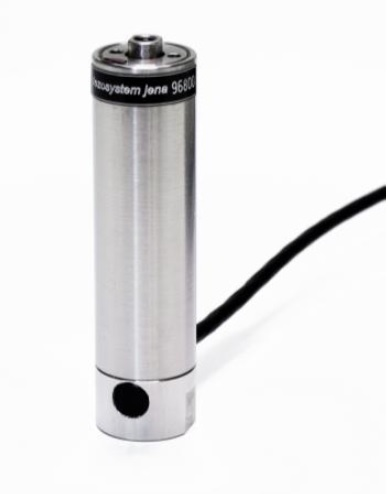
\includegraphics[width=5cm]{Zdjecia/2/piezo_stos}
                \subcaption{\label{subfigure_a}}
        \end{subfigure}
        \begin{subfigure}{0.35\textwidth}
                \centering
	     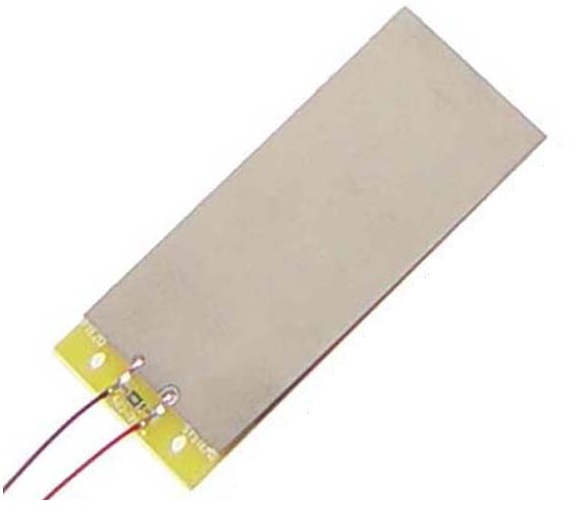
\includegraphics[width=5cm]{Zdjecia/2/piezo_plytka}
                \subcaption{\label{subfigure_b}}
        \end{subfigure}
        \caption{Przetworniki piezoelektryczne: \protect\subref{subfigure_a} w formie sotsu, \protect\subref{subfigure_b} w formie płytki}
        \label{fig:piezoelektryki}
\end{figure}

\vspace{3mm}

Innym sposobem badań jest wykorzystanie techniki laserowej. Za pomocą wiązki lasera możliwe jest wzbudzenie fali sprężystych w materiale. Na szczególną uwagę zasługuje możliwość wzbudzenia fali krótki impulsem, którego widmo będzie miała bardzo duży zakres częstotliwości. Sygnał taki możemy porównać do delty Diraca, dla której widmo ma stałą amplitudę. 

Za pomocą lasera możemy wykonywać także pomiary drgań materiału. Posłużyć może do tego na przykład interferometr laserow, wykorzystujący efekt Dopplera. Detekcja jest jednak ograniczona do fal powierzchniowych. Atutem takiego pomiaru jest możliwość wykonania go dla wielu punktów na badanym obiekcie. Dzięki temu możemy uzyskać przestrzenny obraz propagacji fali.

Przykładowe stanowisko do badania płyt za pomocą wymuszenia laserem przedstawia rysunek \ref{fig:laser}.

\begin{figure}[h]
\centering
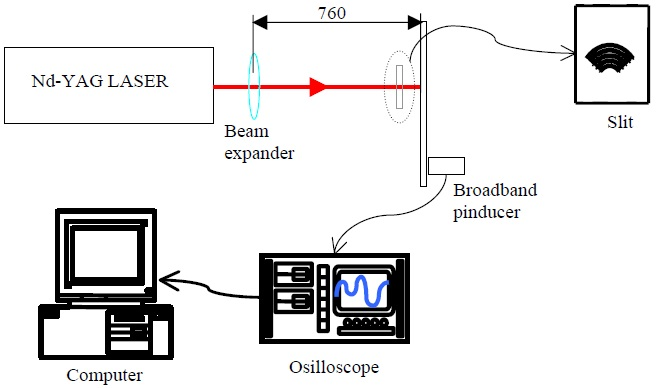
\includegraphics[width=10cm]{Zdjecia/2/laser}
\caption{Przykładowy układ stanowiska do badania fal Lamba w cienkiej płycie \cite{bartek_tian}}
\label{fig:laser}
\end{figure}